\documentclass[twocolumn,11pt]{article}
\setlength{\textheight}{9truein}
\setlength{\topmargin}{-0.9truein}
\setlength{\parindent}{0pt}
\setlength{\parskip}{10pt}
\setlength{\columnsep}{.4in}

\usepackage{amsmath,amsfonts,amssymb,amsthm,bm,caption,calc,ifthen,graphicx,url,hyperref}

\begin{document}
\pagestyle{plain}
\onecolumn
ASTP720 
\newline Homework 2
\newline Will Wainwright
\newline Repository: \href{https://github.com/wjwainwright/ASTP720}{https://github.com/wjwainwright/ASTP720}

\section*{Writeup}
I think the implementation of the rootmt the cubic sp raylem 3, I used root finding instead of interpolation. Forbda methods before. I was able to implement liodsnear interpolation but struggled to implemen 4 and 5at tracing and root findinersg is y straight forward, though I had not really used lae time on this ho, I believe mying to imptowards ource behind the lens. I think that I spent far mor fia point snding methods was prett working correctly, as it appears thmework tryline method. For prob the lines convelement the equations for lensing than I did writing the root finding and interpolation meth.

\begin{figure}[!h]
	\centering
	\noindent
	\makebox[\textwidth]{
      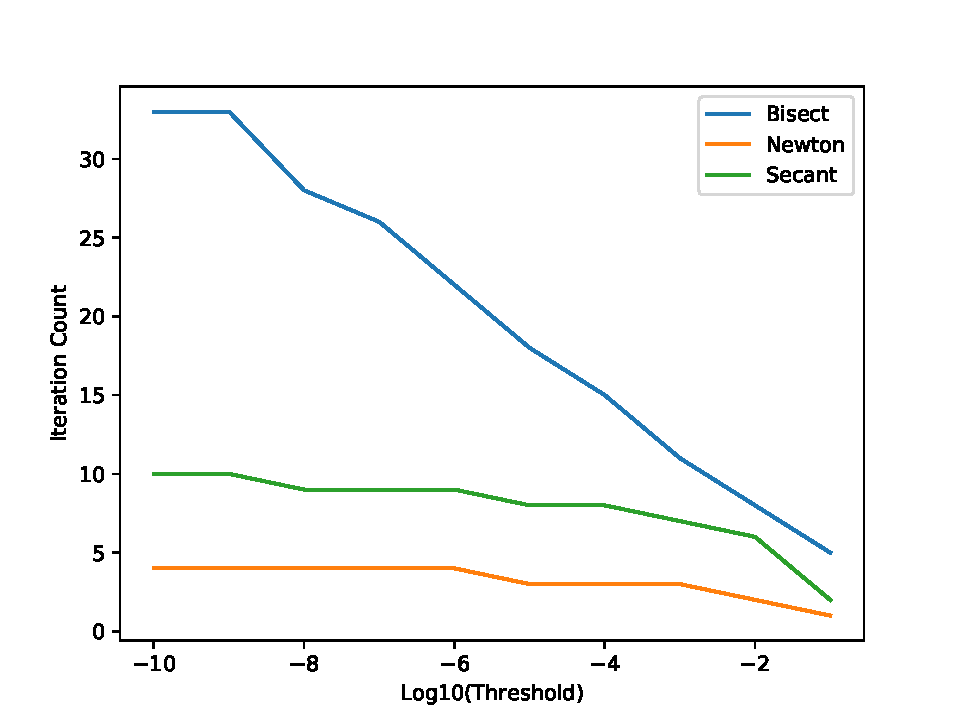
\includegraphics[width=5.5in]{Threshold_Count_Plot.pdf}}
      \caption{}
\end{figure}


\end{document}